\section*{Main HW3 Baseline}

All extra-credit experiments build on the core assignment (\texttt{hw3-1.ipynb}): an unconditioned \texttt{EmojiViT} (4.8M params) trained with weighted \textbf{x-prediction} loss and logit-normal time sampling, then sampled with \textbf{Euler integration} ($T=100$). This is our reference configuration.

\subsection*{Training Results (500 epochs)}

\begin{table}[h]
\centering
\begin{tabular}{l c c c}
\toprule
\textbf{Setting} & \textbf{Final Train Loss} & \textbf{Final Val Loss} & \textbf{Epochs} \\
\midrule
Main HW3 (\texttt{hw3-1}) & 0.1531 & 0.1857 & 500 \\
\bottomrule
\end{tabular}
\caption{Main assignment baseline after full training run.}
\label{tab:main_hw3}
\end{table}

At epoch 300 (where most EC runs stop), the main model reached train $= 0.1747$, val $= 0.1908$---nearly identical to EC re-trains at the same checkpoint, confirming EC baselines reproduce the main HW3 setup.

\begin{figure}[h]
    \centering
    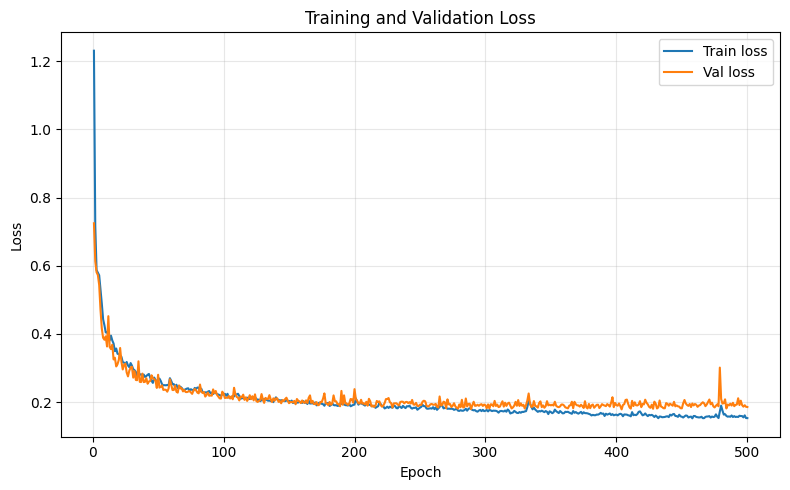
\includegraphics[width=0.75\textwidth]{figures/hw3_main_loss.png}
    \caption{Main HW3 train/validation loss curve (500 epochs).}
    \label{fig:main_loss}
\end{figure}

\begin{figure}[h]
    \centering
    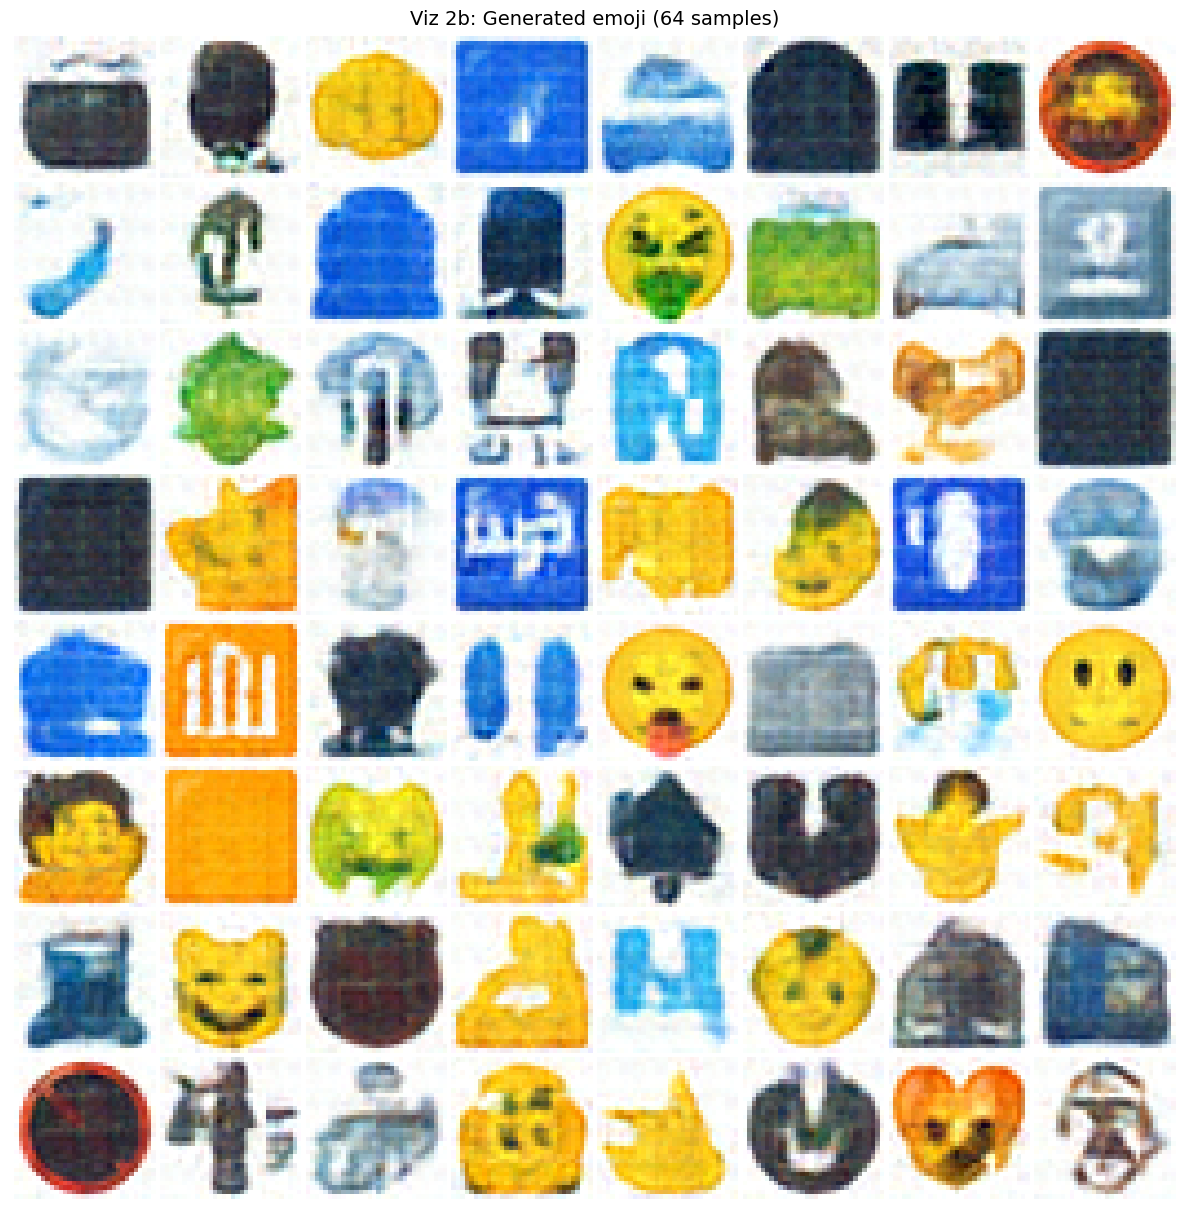
\includegraphics[width=0.65\textwidth]{figures/hw3_main_samples.png}
    \caption{Main HW3 generated emoji (64 samples, Euler $T=100$).}
    \label{fig:main_samples}
\end{figure}

Each EC section below compares against this baseline: EC1 adds time conditioning on top of it; EC2 ablates its x-prediction parameterization; EC3 improves its Euler sampler; EC7 asks whether a model trained this way memorizes or generalizes.
